\chapter{panda-re}

\textbf{Panda-re} or just \textbf{PANDA} (\textbf{P}latform  for  \textbf{A}rchitecture-\textbf{N}eutral  \textbf{D}ynamic  \textbf{A}nalysis) is a framework based on QEMU which provides a programmatic interface to perform deep virtual machine and operating system introspection. It has been designed to be a platform to perform reverse engineering of complex pieces of malware thanks to its ability to record and replay executions. However the functionality is obviously not limited to malware analysis but this framework can be used in all those cases requiring a deep understanding of how a software works or a specific type of analysis such as taint analysis. The typical workflow when using \textbf{PANDA} can be seen in Figure \ref{fig:wkflow}.

\begin{figure}[htp]
\centering
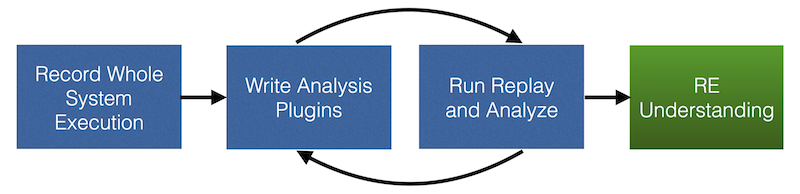
\includegraphics[width=\linewidth]{images/panda_workflow.png}
\caption{Typical panda workflow as desciribed in the documentation.}
\label{fig:wkflow}
\end{figure}


\section{Framework overview}

\textbf{PANDA} leverages the full system emulation capabilities of QEMU, this supports 13 types of CPU architectures while \textbf{PANDA} has built in support for 3 of them: x86, powerPC and ARM. 

Building on top of QEMU architecture \textbf{PANDA} exposes an interface to control the Virtual Machine internal state as well as to access all code and data on the guest operating system. In this way different techniques such as Taint Analysis or Operating System Introspection can be applied.

One of the main components of the framework are \textbf{callbacks}, these are essentially functions that are called when specific events happens inside the virtual machine. Each \textbf{callbacks} is usually called before and after the define event takes place, the relevant function can be selected by using the \textit{before} or \textit{after} prefix (e.g. \lstinline{before_block_exec} and \lstinline{after_block_exec}).

An exhaustive list of available \textbf{callbacks} can be found in the documentation\footnote{\url{https://github.com/panda-re/panda/blob/master/panda/docs/manual.md#appendix-a-callback-list}} however they can be conceptually divided into 4 main categories:

\begin{itemize}
    \item \textbf{Execution Callbacks} are generic callbacks used to trace execution of code inside the virtual machine. There are different levels of granularity that this callbacks provide reflecting events inside the virtual machine, usually at CPU level. Example of this events are: asid change, block execution, block translation or single instruction.
    \item \textbf{Memory Callbacks}, which must be enabled on demand, are called when there is an interaction with the virtual or physical memory. 
    \item \textbf{Replay Only Callbacks} are executed only during replays and usually utilized to handle things like DMA, network interaction and similar.
    \item \textbf{Management Callbacks} are used to perform actions when specific actions related to QEMU takes place, for example when the monitor interface is used.
\end{itemize}

A visual representation of the emulation stage at which the various callbacks are executed can be seen in Figure \ref{fig:calls}.

\begin{figure}[htp]
\centering
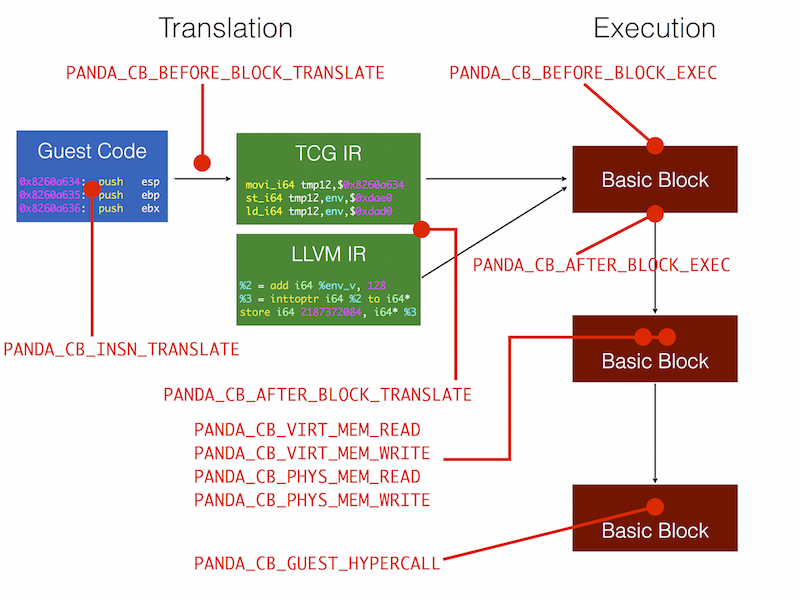
\includegraphics[width=\linewidth]{images/callback_diagram.png}
\caption{Main callbacks and different triggering points. }
\label{fig:calls}
\end{figure}

In addition to callbacks there are some helper functions that are exposed by \textbf{PANDA} in order to make the interaction with QEMU easier. The CPU internal state is saved in a structure called \lstinline{CPUState}, at each time of the execution this structure is made available through a global pointer called \lstinline{env}. 

Moreover \textbf{PANDA} exposes two functions to interact with the Virtual Machine memory: 
\begin{enumerate}
    \item \lstinline{int panda_physical_memory_rw(target_phys_addr_t addr, uint8_t *buf, int len, int is_write);} allowing to read or write bytes, according to the \lstinline{is_write} parameter, at \lstinline{addr} in the pysical memory.
    \item \lstinline{int panda_virtual_memory_rw(CPUState *env, target_ulong addr, uint8_t *buf, int len, int is_write);} which is the same as the above function but used to operate on virtual addresses.
\end{enumerate}


In addition to the above \textbf{PANDA} itself provides some default plugins to perform many different tasks and that can be used as the foundation to further expand analysis capabilities.


\subsection{Plugin system}

The plugin system is the heart of PANDA, a plugin is a piece of code which extends panda functionalities in order to perform specific actions on the running system. Usually a plugin observe the what is happening in the system and either exposes some \textbf{callbacks} that can be used by other plugins or prints information to the user.

\textbf{Callbacks} exposed by a plugin in order to be used by another are called plugin to plugin interface (or \textbf{PPP}) such system allows for the creation of low level plugins that are responsible only to add more functionalities into the \textbf{PANDA} environment, example of such plugins are hooks, syscalls2 or OSI. These are useless if not used in combination with a custom code that takes care of using the \textbf{PPP} exposed by each of them to perform specific actions at well defined execution points.

As it can be easily understood plugins can also be used in combination with helper function to alter the Virtual Machine internal state at run time. As a matter of fact every single component of the VM can be accessed both in read and write mode and this gives the ability to the user to precisely control the execution flow or to introduce custom code or data inside the system whith minimal interaction with it. 


\subsubsection{Plugin writing}

Plugins can be written in C or C++, in order for them to be compiled and enable into PANDA a specific folder structure is required. Such structure is outlined in \ref{fig:plugs}

\begin{figure}[htp]
\centering
\begin{minipage}{\linewidth}
\dirtree{%
.1 panda.
.2 panda.
.3 plugins.
.4 my plugin.
.5 Makefile.
.5 README.md.
.5 myplugin.c.
.4 config.panda.
}
\end{minipage}
\caption{Plugins folder structure}
\label{fig:plugs}
\end{figure}

The Makefile is most of the time standard and provided by PANDA, it can be seen in Figure \ref{fig:mak}

\begin{figure}[htp]
\centering
\begin{minipage}{\linewidth}
\begin{lstlisting}
# Don't forget to add your plugin to config.panda!

# If you need custom CFLAGS or LIBS, set them up here
# CFLAGS+=
# LIBS+=

# The main rule for your plugin. List all object-file dependencies.
$(PLUGIN_TARGET_DIR)/panda_$(PLUGIN_NAME).so: \
	$(PLUGIN_OBJ_DIR)/$(PLUGIN_NAME).o
\end{lstlisting}
\end{minipage}
\caption{Basic Makefile}
\label{fig:mak}
\end{figure}

Moreover each plugin should expose at least the following two functions: \lstinline{bool init_plugin(void *)} \lstinline{void uninit_plugin(void *)}.

The first one is called during plugin initialisation and is where the different functions and callbacks are initialized. The second one is called when panda is terminating or when the plugin is unloaded and is typically used to clean up custom structures initialized by the plugin.

In addition to this the plugin should import the following file \lstinline{#include "panda/plugin.h"} which is essentially the \textbf{PANDA} API. Lastly the name of the plugin should be added to the \lstinline{config.panda} file in order for it to be automatically compiled during panda compilation.


\subsection{Record and Replay}

In addition to the above plugin system \textbf{PANDA} also features a method to record the entire state of the machine and replay that later in a deterministic way. This leverages the \textbf{rr} (record and replay) framework from Mozilla which was usually developed to extend gdb functionalities and allow for time travel debugging. 

\textit{"You record a failure once, then debug the recording, deterministically, as many times as you want. The same execution is replayed every time."}\footnote{\url{https://rr-project.org/}}

This enables writing complex and articulated plugins and allows for faster analysis, as a matter of fact plugins introduce overhead in the execution. Recording the execution of a malware without any plugins enabled and then run them on the recording allows to get rid of a lot of that overhead. This is the typical workflow as in Figure \ref{fig:wkflow}. Due to the fact that the replay is deterministic it will have the same result at every run. It means that the results are the same as if the machine is booted up, the OS is started and initialized, possibly some modifications applied and then run the program to be analyzed. This has however some limitations as explained on the\textbf{rr} website: 

\textit{"Unlike many record and replay implementations, we do not record the inputs to devices; this means that one cannot "go live" during a recording, but it greatly simplifies the implementation. To get an idea of what is recorded, imagine drawing a line around the CPU and RAM; things going from the outside world to the CPU and RAM, crossing this line, must be recorded."}

A recording can be taken via the QEMU monitor interface using the \lstinline{begin_record <replay name>} and \lstinline{end_record} commands, this will create two files: \lstinline{<replay name>-rr-snp} which is a snapshot of the VM at the beginning of the recording and \lstinline{<replay name>-rr-nondet.log} which will hold a log of all non deterministic inputs during the recording. A recording can then be replayed by adding the \lstinline{-replay <replay name>} command line argument to the panda executable. 

Plugins are generally used for analysis therefore they rarely modify directly the virtual machine environment but instead they focus on catching particular behaviours and logging it or perform some more analysis based on specific events happening inside the virtual machine. As mentioned before in order for the replay functionality to be used it is important that the plugin doesn't alter the control flow of the program, as a matter of fact due to the nature of \textit{rr} (\underline{deterministic} record and replay) if a replayed trace diverges from what has been recorder (for example the program takes a different conditional jump) it will no longer be able to continue the replay as it will not be able to find what should be replayed anymore. For this reason plugins that introduce modifications in the virtual machine, such as hiding specific virtualization artifacts, must be run on the live system. In the same way it is not possible to perform analysis that will make the execution diverge from the recording, this means for example that during the analysis of a malware the Command and Control communications must be deterministic and is not possible to record just 1 interaction with the C2 and then bruteforce all the possible commands during the replay.


\subsection{Python bindings}

In addition to the above mentioned plugins system \textbf{PANDA} exposes also a Python interface, this is referred to as \textbf{pypanda}. The documentation for the python package can be found at \url{https://panda-re.github.io/panda.html}. Such interface allows for better scriptability and to have faster prototyping. Everything that can be done with a "standard" C/C++ plugin can be accomplished with Python moreover, \textbf{pypanda} exposes some high level functions that can be used to write entire scripts to automatically run a self contained simulation.

In addition to this there are some C/C++ plugins created to be used specifically with \textbf{pypanda}, for example the hooks plugin, as mentioned in issue 613\footnote{\url{https://github.com/panda-re/panda/issues/613}}:

\textit{"It's designed to be used with the python interface which has some code to ensure the hook only runs when in the right process so you'd either need to reimplement that logic or use the python interface"}

While proper plugins are somehow specialized pieces of code designed to analyze or act on a specific behaviour python code can interact directly with \textbf{PANDA} and can be used not only to build new plugins but also to control the entire simulation life cycle without the user having to interact with the command line or on the qemu monitor.

\textbf{pypanda} exposes a class used to interact with \textbf{PANDA}: \lstinline{class Panda (arch='i386', mem='3G', expect_prompt=None, os_version=None, qcow=None, os='windows', generic=None, raw_monitor=False, extra_args=[])}, this accepts different parameters to create a well defined virtual machine. The newly created VM can then be used to run either a live system or a recording, obviously if run on the recording this should have been taken on a VM with the same system configuration. 

There is a small overhead when utilizing \textbf{pypanda} due to the nature and efficiency of the python code which is naturally different from pure C/C++ implementations however, as mentioned before, there are some operations such as setting hooks that are designed to be done mainly via the python interface. Moreover the python library exposes some more convenient methods to access internal structures compared with classical \textbf{PANDA} APIs. 

From the python interface it is possible to access not only \textbf{PPP} interfaces but also classical python callback, this as mentioned before allows for very complex interactions to be written in python. As a matter of fact there are different helper functions such as \lstinline{get_mappings, get_process_name, ...} that provides direct interfaces to other plugins such as OSI, hooks, taint and others. The function \lstinline{run} or \lstinline{run_replay} can then be used to run the simulation. Other helper functions include \lstinline{record} and \lstinline{end_record} used to control the recording, this allows to write python scripts that automatically run a simulation on the live system, records it, then runs some specific plugins on the recording. 

\section{Advantages compared to its competitors}
\todo{A lot of features, nice interface, record and replay}
There are other similar projects such as TEMU, DECAF and DRAKWUF however PANDA has some advantages and useful functionalities that can be helpful for analyzing evasive malware and to implement a sthealt VM.

One of the most interesting features of PANDA is the ability to record and replay execution. In particular in relation to evasive malware this is useful as it is possible to write a plugin to hide virtualization artifacts from the system and then run a malware on such system recording its execution. Others plugins can then be used on the replay to perform a proper malware analysis. 

Moreover exposing a python interface, although this introduces a bit of overhead, is a great feature compared to the other frameworks which allows for great scriptablility of actions and fast prototyping of complex experiments.